\documentclass[resume]{subfiles}


\begin{document}
    \section{Résolution numérique de systèmes linéaires}
\paragraph{Système mal conditionné} $\kappa_\infty(A)$ très grand     
    
    \begin{align*}
    a_{11}x_1+\cdots+a_{1n}x_n &=b_1\\
    \vdots \\
    a_{n1}x_1 + \cdots + a_{nn}x_n &= b_n
    \end{align*}
    
    $$\underbrace{\begin{pmatrix}
    a_{11} & \cdots & a_{1n}\\
    \vdots & \ddots & \vdots\\
    a_{n1} & \cdots & a_{nn}
    \end{pmatrix}}_{A}\underbrace{\begin{pmatrix}
    x_1\\\vdots\\x_n
    \end{pmatrix}}_{\vec{x}}=\underbrace{\begin{pmatrix}
    b_1\\\vdots\\b_n
    \end{pmatrix}}_{\vec{b}}$$
	Si peu d'éléments sont non-nuls alors $A$ est dite \textbf{creuse}
	\subsection{Condition d'arrêt}
	$$\boxed{\abs{\abs{\vec{r}_k}}=\abs{\abs{\vec{b}-A\vec{x}_k}}}$$
	Tolérance fixe $\tau$ (par exemple $10^{-5}$)
	$$\abs{\abs{\vec{r}_k}}\leq \tau\abs{\abs{\vec{b}}}$$
	Erreur :
	$$\vec{e}_k=\vec{x}-\vec{x}_k$$
	On peut aussi utiliser une condition d'arrêt sur l'erreur $\vec{e}_k$ au lieu du résidu $\vec{r}_k=\vec{b}-A\vec{x}_k$
	\subsubsection{Lien entre résidu et erreur}
	$$\frac{\abs{\abs{\vec{x}-\vec{x}_k}}}{\abs{\abs{\vec{x}_k}}_p}\leq \underbrace{\abs{\abs{A}}_p\abs{\abs{A^{-1}}}_p}_{\kappa_p(A)}\frac{\abs{\abs{\vec{b}-A\vec{x}_k}}_p}{\abs{\abs{\vec{b}}}_p}$$
	Autant de digits valides dans la mantisse que
	$$N_\text{digits}=\abs{\log_{10}(\varepsilon)}-\log_{10}(\kappa(A)_p)$$
	Avec $\varepsilon$ la précision machine (1e-16 en général)
	\subsubsection{Perturbation}
	Perturbation sur $A$
	$$\boxed{\frac{\abs{\abs{\delta\vec{x}_A}}}{\abs{\abs{\vec{x}+\delta \vec{x}_A}}}\leq \abs{\abs{\vec{A}}}\cdot\abs{\abs{\vec{A}^{-1}}}\cdot\frac{\abs{\abs{\delta A}}}{\abs{\abs{A}}}}$$
	Perturbation sur $A$ et $\vec{b}$:
	\begin{small}
	$$\boxed{\frac{\abs{\abs{\delta\vec{x}}}}{\abs{\abs{\vec{x}+\delta \vec{x}}}}\leq \frac{\abs{\abs{\vec{A}}}\cdot\abs{\abs{\vec{A}^{-1}}}}{1-\abs{\abs{A}}\cdot \abs{\abs{A^{-1}}}\frac{\abs{\abs{\delta A}}}{\abs{\abs{A}}}}\cdot\left(\frac{\abs{\abs{\delta A}}}{\abs{\abs{A}}}+\frac{\abs{\abs{\delta \vec{b}}}}{\abs{\abs{\vec{b}}}}\right)}$$
	\end{small}
	\subsection{Normes}
	$$\abs{\abs{\vec{v}}}_p=\left(\sum_{i=1}^{n}\abs{v_i}^p\right)^{\frac{1}{p}}$$
	\begin{enumerate}
	\item Vecteurs
		\begin{enumerate}
	\item 1-norme : somme des composantes
	\item 2-norme : norme euclidienne
	\item max-norme : $p\to\infty$ max des valeurs absolues
%	$$\abs{\abs{\vec{v}}}_{\infty}=\max(\abs{v_i})$$
	\end{enumerate}
	\item Matrices
	\begin{enumerate}
	\item 1-norme : $\max\left(\sum\abs{A}\right)$ (la somme est colonne par colonne).
%	$$\abs{\abs{A}}_1=\max_{1\leq j\leq n}\sum_{i=1}^{n}\abs{a_{ij}}$$
	\item 2-norme : ou max des valeurs propres de $A^{T}A$
%	$$\abs{\abs{A}}_2=\sqrt{\max\abs{\lambda(A^{T}A)}}$$
	\item max-norme : $\max\left(\sum\abs{A}\right)$ (la somme est ligne par ligne).
%	$$\abs{\abs{A}}_{\infty}=\abs{\abs{A^{T}}}_1$$
	\end{enumerate}
	\end{enumerate}

	\begin{enumerate}
	\item $\abs{\abs{\vec{v}}}=0\longleftrightarrow \vec{v}=\vec{0}$
	\item $\abs{\abs{\lambda\vec{v}}}=\abs{\lambda}\cdot \abs{\abs{\vec{v}}}$
	\item $\abs{\abs{\vec{v}+\vec{u}}}\leq \abs{\abs{\vec{v}}}+\abs{\abs{\vec{u}}}$
	\end{enumerate}
	\subsection{Méthodes directes}
	\subsubsection{Élimination de Gauss sans pivot}
	Effectuer des combinaisons linéaires des lignes pour obtenir une matrice triangulaire supérieure. Matrice augmentée :
	$$\begin{amatrix}{3}
10 & -7 & 0 & 7\\
0 & -0.1 & 6 & 6.1\\
0 & 2.5 & 5 & 2.5\\
\end{amatrix}$$
\begin{enumerate}
\item Commencer par la colonne de gauche
\item Si nécessaire, permuter les lignes pour avoir un non-nul comme premier élément
\item Faire les combinaisons linéaires des lignes pour annuler les éléments inférieurs
\item Passer à la colonne suivante
\end{enumerate}
\subsubsection{Élimination de Gauss avec pivot}
On fait le premier pas normalement (0 en dessous du premier élément). Mais avant d'effectuer le prochain pas, on échange les lignes pour avoir le plus grand élément en diagonale. A la fin on se retrouve avec, par exemple :
$$A=\begin{pmatrix}
10 & x & x\\
0 & 6 & x\\
0 & 0 & 0.01
\end{pmatrix}$$
\subsection{LU}
$$A\vec{x}=\vec{b}\longrightarrow L\underbrace{U\vec{x}}_{\vec{y}}=\vec{b}$$
L'avantage est que si on change $b$, il n'y a pas besoin de tout recommencer.
\paragraph{Avec pivotement}
Si on applique le pivotement, on a une matrice de permutation $P$
$$LU=PA$$
\subsubsection{Doolittle}
Méthode équivalente à l'élimination de Gauss
$$\begin{pmatrix}
a_{11} & a_{12} & a_{13}\\
a_{21} & a_{22} & a_{23}\\
a_{31} & a_{32} & a_{33}
\end{pmatrix}=\begin{pmatrix}
1 & 0 & 0\\
l_{21} & 1 & 0\\
l_{31} & l_{32} & 1
\end{pmatrix}\begin{pmatrix}
u_{11} & u_{12} & u_{13}\\
0 & u_{22} & u_{23}\\
0 & 0 & u_{33}
\end{pmatrix}$$
\begin{figure}[H]
\centering
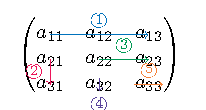
\includegraphics[scale=1,page=1]{drwg_6.pdf}
\end{figure}
\begin{align*}
(1)&\begin{cases}
u_{11}&=a_{11}\\
u_{12}&=a_{12}\\
u_{13}&=a_{13}
\end{cases} \qquad (2)\begin{cases}
l_{21}&=\frac{a_{21}}{u_{11}}\\
l_{31}&=\frac{a_{31}}{u_{11}}
\end{cases}\\
(3)&\begin{cases}
u_{22}&=a_{22}-l_{21}u_{12}\\
u_{23}&=a_{23}-l_{21}u_{13}
\end{cases} \qquad(4)\begin{cases}
l_{32}=\frac{a_{32}-l_{31}u_{12}}{u_{22}}
\end{cases}\\
(5)&\begin{cases}u_{33}=a_{33}-l_{31}u_{13}-l_{32}u_{23}\end{cases}
\end{align*}
Formules générales (au cas ou matrice plus petite ou plus grande) :
$$u_{km}=a_{km}-\sum_{j=1}^{k-1}l_{kj}u_{jm}\qquad m=k,k+1,k+2,...,n$$
$$l_{ik}=\frac{1}{u_{kk}}\left(a_{ik}-\sum_{j=1}^{k-1}l_{ij}u_{jk}\right)\qquad i=k+1,k+2,...$$
\subsubsection{Cholesky}
$$\begin{pmatrix}
a_{11} & a_{12} & a_{13}\\
a_{12} & a_{22} & a_{23}\\
a_{13} & a_{23} & a_{33}
\end{pmatrix}=\begin{pmatrix}
\hat{l}_{11} & 0 & 0\\
\hat{l}_{21} & \hat{l}_{22} & 0\\
\hat{l}_{31} & \hat{l}_{32} & \tilde{l}_{33}
\end{pmatrix}\cdot\begin{pmatrix}
\hat{l}_{11} & \hat{l}_{21} & \hat{l}_{31}\\
0 & \hat{l}_{22} & \hat{l}_{32}\\
0 & 0 & \tilde{l}_{33}
\end{pmatrix}$$
\begin{align*}
\hat{l}_{11}&=\sqrt{a_{11}} & \hat{l}_{21}&=\frac{a_{12}}{\sqrt{a_{11}}}\\
\hat{l}_{31}&=\frac{a_{13}}{\sqrt{a_{11}}} & \hat{l}_{22}&=\sqrt{a_{22}-\frac{a_{12}}{\sqrt{a_{11}}}}\\
\hat{l}_{32}&=\frac{a_{23}-\frac{a_{13}a_{12}}{a_{11}}}{\sqrt{a_{22}-\frac{a_{12}}{a_{11}}}} & \hat{l}_{33}&=\sqrt{a_{33}-\hat{l}_{31}^2-\hat{l}_{32}^2}
\end{align*}
\subsubsection{Permutations}
Attention, si on utilise des permutations, alors
$$PA\vec{x}=P\vec{b}$$
\subsubsection{Méthode QR}
$R$ est triangulaire supérieur (en dessous-gauche de la diagonale : que des 0)
$$A=QR\longrightarrow R\vec{x}=Q^{-1}\vec{b}\longrightarrow R\vec{x}=\underbrace{Q_t\vec{b}}_{\vec{c}}$$
\begin{scriptsize}
$$\begin{pmatrix}
\\
\vec{a}_1 & \cdots & \vec{a}_n\\
\\
\end{pmatrix}=\begin{pmatrix}\\
\vec{q}_1 & \cdots & \vec{q}_m\\
\\
\end{pmatrix}\begin{pmatrix}
r_{11} & r_{12} & \cdots & r_{1n}\\
0 & r_{22} & \cdots & r_{2n}\\
\vdots & \vdots & \ddots & \vdots\\
0 & 0 & \cdots & r_{nn}\\
0 & 0 & \cdots & 0
\end{pmatrix}$$
\end{scriptsize}
Avec les propriétés de $Q$ :
\begin{itemize}
\item $Q^TQ=I\quad Q^{-1}=Q^T$
\item $\det(Q)=\pm 1$
\end{itemize}







On commence avec une matrice $A_{n\times n}$
\begin{enumerate}
\item Prendre le premier vecteur colonne de $A$ : $\vec{x}_1$
\item Déterminer $\vec{y}$
$$y=\textcolor{OrangeRed}{-}\rho\begin{pmatrix}
1\\0\\\vdots\\0
\end{pmatrix}=\textcolor{OrangeRed}{-}\text{signe}(a_{ii})\abs{\abs{x_i}}\left.\begin{pmatrix}
1\\0\\\vdots\\0
\end{pmatrix}\right\rbrace\text{taille de }x$$
\item Déterminer $\vec{v}$
$$\vec{v}=\vec{x}-\vec{y}$$
$$\gamma=\frac{\abs{\abs{\vec{v}}}^2}{2}$$
\item Faire la décomposition pour obtenir $H_1$
$$\tilde{H}=I-\frac{2}{\abs{\abs{v}}^2}vv^T$$
$$H=\begin{pmatrix}
I & 0\\
0 & \tilde{H}
\end{pmatrix}\quad \text{(si nécessaire)}$$

\item Construire $H_1A$ puis prendre $v_2$ (première colonne de $H_1A$ \textbf{sans la première ligne et sans la première colonne}
\item Recommencer jusqu'à avoir terminé
\item à la fin, déterminer $R$ et $Q$
\end{enumerate}
$$H_nH_{n-1}\cdots H_2H_1A=R\longrightarrow A=\underbrace{H_1H_2\cdots H_{n-1}^TH_n^T}_{Q}R$$

\subsubsection{Système creux} : Réseaux hydrauliques, thermiques, électriques, etc... Possibilité de faire du "fill-in" si $n$ ou $b$ sont grands mais le coup sera inutilement grand.
\subsubsection{Valeur $\kappa$}
$$\kappa(A)_p=\abs{\abs{A}}_p\abs{\abs{A^{-1}}}_p$$
En général on utilisera $\kappa_2$ si ce n'est pas précisé (mais des fois on calcule $\kappa_\infty$)
\subsection{Résolution au sens des moindres carrés}
On résout le système
$$A^TA\vec{x}=A^T\vec{b}$$
Si $A$ est mal conditionné, $A^TA$ est doublement mal conditionné
$$\kappa(A^TA)\approx\kappa^2(A)$$
Pour obtenir le nombre de digits corrects, on fait :
$$N_\text{digits}=\abs{\log_{10}(\epsilon)}-\log_{10}(\kappa)$$
Avec $QR$ , on a une méthode plus stable
$$\underset{m\times n}{A}=\underset{m\times m}{Q}\underset{m\times n}{\begin{pmatrix}R^\ast\\ 0\end{pmatrix}}$$
\subsubsection{Minimisation}
$$\abs{\abs{\vec{b}-A\vec{x}}}=\abs{\abs{QQ^T\vec{b}-QR\vec{x}}}=\abs{\abs{\underbrace{Q^T\vec{b}}_{\vec{c}}-R\vec{x}}}$$
\begin{enumerate}
\item Trouver $Q$ et $R$ avec la méthode au dessus
\item Calculer $\vec{c}$
$$\vec{c}=Q^T\vec{b}$$
\item Trouver $R^\ast$ (partie "supérieure" de $R$, donc sans les 0 en bas)
\item Trouver $c^\ast$ (partie "supérieure" de $\vec{c}$, en ignorant la valeur du bas pour avoir la même hauteur que $R^\ast$)
\item Poser le système
$$R^\ast\vec{x}=\vec{c}^\ast$$
\item Résoudre à la main, en inversant, c'est égal
\end{enumerate}
\subsection{Méthodes itératives}
\begin{figure}[H]
\centering
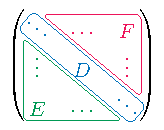
\includegraphics[scale=1,page=1]{drwg_2.pdf}
\end{figure}
\subsubsection{Méthode Jacobi}
On commence avec un $\vec{x}(0)=\vec{0}$
$$x_i^{(k+1)}=\frac{1}{a_{ii}}\left(b_i-\sum_{j\neq i}a_{ij}x_j^{(k)}\right)$$
\begin{small}
$$\boxed{\begin{pmatrix}x_1\\x_2\\\vdots\\x_n\end{pmatrix}^{(k+1)}=\begin{pmatrix}
\frac{1}{a_{11}}\cdot(b_1-a_{12}x_2^{(k)} \cdots -a_{1n}x_n^{(k)})\\
\frac{1}{a_{22}}\cdot(b_2-a_{21}x_1^{(k)} \cdots -a_{2n}x_n^{(k)})\\
\vdots\\
\frac{1}{a_{nn}}\cdot(b_n-a_{n1}x_1^{(k)} \cdots -a_{n\ n-1}x_{n-1}^{(k)})
\end{pmatrix}}$$
\end{small}
Alternativement :
$$\boxed{\vec{x}^{(k)}=D^{-1}\left(b-(A-D)\vec{x}^{(k-1)}\right)}$$
$$N=D^{-1}=\text{diag}^{-1}(A)$$
Convergence assurée sur $A$ est \textbf{strictement diagonalement dominante}\ref{strict_diag_dom}
\subsubsection{Méthode de Gauss-Seidel}
$$x_i^{(k+1)}=\frac{1}{a_{ii}}\left(b_i-\sum_{j=1}^{i-1}a_{ij}x_j^{(k+1)}-\sum_{j=i+1}^{n}a_{ij}x_j^{(k)}\right)$$
\begin{small}
$$\boxed{\overset{(k+1)}{\begin{pmatrix}x_1\\x_2\\\vdots\\x_n\end{pmatrix}}=\begin{pmatrix}
\frac{1}{a_{11}}\cdot(b_1-a_{12}x_2^{(k)} \cdots -a_{1n}x_n^{(k)})\\
\frac{1}{a_{22}}\cdot(b_2-a_{21}x_1^{(k+1)} \cdots -a_{2n}x_n^{(k)})\\
\vdots\\
\frac{1}{a_{nn}}\cdot(b_n-a_{n1}x_1^{(k+1)} \cdots -a_{nn-1}x_n^{(k+1)})
\end{pmatrix}}$$
\end{small}
Alternativement :
$$\boxed{\vec{x}^{(k)}=(E+D)^{-1}\left(\vec{b}-F\vec{x}^{(k-1)}\right)}$$
$$N=(D+E)^{-1}$$
Gauss-Seidel est bien meilleur que la méthode de Jacobi.\\
Convergence assurée sur $A$ est \textbf{strictement diagonalement dominante}\ref{strict_diag_dom}

\subsubsection{Méthode SOR}
$$\vec{x}^{(k+1)}=(D+\omega E)^{-1}\cdot \left(\omega \vec{b}-(\omega F+(\omega-1)D)\vec{x}^{(k)}\right)$$
\subsubsection{Itération simple}
$$\vec{x}^{(k+1)}=\vec{x}^{(k)}+N\left(\vec{b}-A\vec{x}^{(k)}\right)$$
$$\max_i\abs{\lambda_i}<1\longrightarrow\text{ convergence assurée pour tout }\vec{b}$$
\subsection{Convergence}
De manière générale on a une expression de la forme
$$\vec{x}^{(k)}=\vec{x}^{(k-1)}+\textcolor{OrangeRed}{N}\left(\vec{b}-A\vec{x}^{(k-1)}\right)$$
Avec un $\textcolor{OrangeRed}{N}$ qui se rapproche de $A^{-1}$ pour que le système soit rapide (mais sans être trop dur à calculer).\\
$$\boxed{\rho(I-NA)=\max\left(\text{valeurs propres}(I-NA)\right)}$$
$$\rho < 1\longrightarrow\text{ convergence garantie}$$
\subsubsection{Erreur}
$$e^{(k)}=\underbrace{(I-NA)}_\text{matrice d'itération}e^{(k-1)}$$
$$\abs{\abs{\vec{e}^{(k)}}}\leq \rho^{k}\abs{\abs{\vec{e}^{(0)}}}$$
Relation entre le nombre de décimales souhaitées $D$ et le nombre d'itérations $n$
$$n\geq \frac{\log_{10}(10^{-D})}{\log_{10}(\rho)}=-\frac{D}{\log_{10}(\rho)}$$
\subsection{Matrice strictement diagonalement dominante}
\label{strict_diag_dom}
$$\sum_{\forall j\neq i}\abs{a_{ij}}<\abs{a_{ii}}$$
$a_{ii}$ est la plus grande valeur sur chaque ligne
\subsection{Méthodes de minimisation $A\vec{x}-\vec{b}$}
$$\boxed{\vec{r}=\vec{b}-Ax}$$
\paragraph{Gradient}
$$\nabla G(\vec{x})=\begin{pmatrix}G_x\\G_y\\G_z\end{pmatrix}$$
Si on multiplie par la transposée de $\vec{n}$ on obtient la dérivée directionnelle.
$$\frac{\partial G}{\partial \vec{n}}=\vec{n}^{T}\nabla G(\vec{x})$$
Il existe deux méthodes de résolutions et deux algorithmes ($F$ fonctionne toujours et $G$ fonctionne si $A$ est symétrique et semi-définie positive, voir définition plus bas) 
\subsubsection{Méthode 1 : $F(x)=\frac{1}{2}\abs{\abs{b-A\vec{x}}}^2_2$}
On cherche à minimiser le résidu $\vec{r}$ (fonctionne seulement si $A\vec{x}=\vec{b}$ possède au moins une solution)
$$\vec{d}=A^T(\vec{b}-A\vec{x})$$
\paragraph{Algorithme de la plus grande pente}
$$\vec{d}_k=-\nabla F=A^T(\vec{b}-A\vec{x}_k)$$
$$\vec{x}_{k+1}=\vec{x}_k+\vec{d}_k$$
\paragraph{Algorithme des gradients conjuguées} (pas sur que cet algorithme peut être utilisé avec cette méthode)
On utilise le résidu précédent et le résidu actuel pour optimiser encore plus l'itération
$$\vec{d}_{k+1}=\vec{r}_{k+1}+\beta_k\vec{d}_k$$
$$\beta=\frac{\vec{r}_{k+1}^T\vec{r}_{k+1}}{\vec{r}_k^T\vec{r}_k}$$
$$\vec{x}_{k+1}=\vec{x}_{k}+\alpha_k\vec{d}_k$$


\subsubsection{Méthode 2 : $G(x)=\frac{1}{2}\vec{x}^TA\vec{x}-\vec{b}^T\vec{x}$}
Deux notations possibles :
$$G(x)=\frac{1}{2}\vec{x}^TA\vec{x}-\vec{x}^T\vec{b}=\frac{1}{2}\vec{x}^TA\vec{x}-\vec{b}^T\vec{x}$$
$A$ doit être semi-définie positive (valeurs propres de $A$ plus grandes ou égales à 0)
$$\vec{x}^TA\vec{x}\geq 0$$
$$\vec{d}=\vec{r}=\vec{b}-A\vec{x}$$
\paragraph{Algorithme de la plus grande pente (zig-zag)}
$$\vec{d}_k=-\nabla F=A^T(\vec{b}-A\vec{x}_k)$$
$$\vec{x}_{k+1}=\vec{x}_k+\vec{d}_k$$
Si on utilise $\alpha$ optimal, alors toutes les itérations sont à angle droit. Calcul de $\alpha$ optimal :
$$\alpha_k=\frac{\vec{d}_k^T\vec{r}_k}{\vec{d}^T_kA\vec{d}_k}$$
\paragraph{Algorithme des gradients conjuguées} (réponse après $n$ itérations, avec $n$ la largeur de la matrice $A$)
On utilise le résidu précédent et le résidu actuel pour optimiser encore plus l'itération
$$\vec{d}_{k+1}=\vec{r}_{k+1}+\beta_k\vec{d}_k$$
$$\beta=\frac{\vec{r}_{k+1}^T\vec{r}_{k+1}}{\vec{r}_k^T\vec{r}_k}$$
$$\vec{x}_{k+1}=\vec{x}_{k}+\alpha_k\vec{d}_k$$

    


    
\end{document}